\documentclass[10pt, a4paper]{article}

%%%%%%%%%%%%%%
%  Packages  %
%%%%%%%%%%%%%%


\usepackage{page_format}
\usepackage{special}
\usepackage{hyperref}
\usepackage{tikz}
\usepackage[compat=1.1.0]{tikz-feynman}
%----------------------------------------------------------------------
%\usepackage{amssymb} % Mathematical fonts.
%\usepackage{amsfonts} % Mathematical fonts.
\usepackage[nice]{nicefrac} % Nicer fractions
\usepackage{braket} % Dirac Notation.
\usepackage{bbm} % More bold fonts.
%\usepackage{mathrsfs} % Mathematical fonts.
\usepackage{esint} % Integrals
\usepackage{cancel} % Allows to scratch expressions.
\usepackage{mathtools} % Tools for math formating.
\usepackage{slashed} % Allows to slash individual characters.
\usepackage{xargs} % Better handling of optional arguments for commands
%----------------------------------------------------------------------
%\usepackage{lmodern} % Fonts.
\usepackage{feyn} % Feynman Diagrams in mathmode

%%%%%%%%%%%%%%%%%%%%%%%%%%%
% Mathématiques et physique
%%%%%%%%%%%%%%%%%%%%%%%%%%%%
% SI Units -----------------------
% The package 'siunitx' causes unresolved crashes (as of 22/08/31)
\newcommand{\ampere}{\text{A}}
\newcommand{\bell}{\text{B}}
\newcommand{\celsius}{\degree\text{C}}
\newcommand{\coulomb}{\text{C}}
\newcommand{\degree}{\,^{\circ}}
\newcommand{\farad}{\text{F}}
\newcommand{\electro}{\text{e}}
\newcommand{\gram}{\text{g}}
\newcommand{\henry}{\text{H}}
\newcommand{\hertz}{\text{Hz}}
\newcommand{\hour}{\text{h}}
\newcommand{\joule}{\text{J}}
\newcommand{\kelvin}{\text{K}}
\newcommand{\meter}{\text{m}}
\newcommand{\minute}{\text{m}}
\newcommand{\mole}{\text{mol}}
\newcommand{\newton}{\text{N}}
\newcommand{\ohm}{\Omega}
\newcommand{\pascal}{\text{Pa}}
\newcommand{\rad}{\text{rad}}
\newcommand{\second}{\text{s}}
\newcommand{\tesla}{\text{T}}
\newcommand{\torr}{\text{Torr}}
\newcommand{\volt}{\text{V}}
\newcommand{\watt}{\text{W}}
%
\newcommand{\tera}{\text{T}}
\newcommand{\giga}{\text{G}}
\newcommand{\mega}{~\text{M}}
\newcommand{\kilo}{~\text{k}}
\newcommand{\deci}{\text{d}}
\newcommand{\centi}{\text{c}}
\newcommand{\milli}{\text{m}}
\newcommand{\micro}{\mu}
\newcommand{\nano}{\text{n}}
\newcommand{\pico}{\text{p}}
\newcommand{\femto}{\text{f}}
%
\newcommand{\units}[1]{\text{#1}}
\newcommand{\tothe}[1]{\textsuperscript{#1}}
%
\newcommand{\per}{\text{/}}
%
\newcommand{\Time}[3]{#1\hour~#2\minute~#3\second} % TODO Optional arguments.
\newcommand{\Angle}[3]{#1^{\circ}~#2'~#3''} % TODO Optional arguments.


% Better epsilon -----------------------
\let\oldepsilon\epsilon
\let\epsilon\varepsilon
\let\varepsilon\oldepsilon


% Better \bar -----------------------
\renewcommand{\bar}[1]{\mkern 1.5mu\overline{\mkern-1.5mu#1\mkern-1.5mu}\mkern 1.5mu}


% Équations -----------------------
\newcommand{\al}[1]{\begin{align} #1 \end{align}} % Numbered equation(s),
\newcommand{\eqn}[1]{\begin{align*} #1 \end{align*}} % Number-less equation(s),
\newcommand{\sys}[1]{\begin{dcases*} #1 \end{dcases*}} % System of equations.


% Exponents -----------------------
\newcommand{\Exp}[1]{\text{e}^{#1}}		% e^#
\newcommand{\E}[1]{\times 10^{#1}}		% X 10^#


% Delimiters -----------------------
\newcommand{\p}[1]{\left( #1 \right)}	% (#)
\newcommand{\cro}[1]{\left[ #1 \right]}	% [#]
\newcommand{\abs}[1]{\left| #1\right|}	% |#|
\newcommand{\avg}[1]{\left\langle #1 \right\rangle} % <#>
\newcommand{\acc}[1]{\left\lbrace #1 \right\rbrace} % {#}


% Vectors -----------------------
\newcommand{\ve}[1]{\mathbf{#1}} % Upright bold face.
\newcommand{\vu}[1]{\hat{\ve{#1}}} % Hat vector upright bold face
\newcommand{\tens}{\otimes} % Tensor product
\newcommand{\nablav}{\bm{\nabla}} % Bold gradient


% Trig. functions with automatic formating  -----------------------
\newcommandx{\Sin}[2][1={}]{\text{sin}^{#1}\!\p{#2}}
\newcommandx{\Cos}[2][1={}]{\text{cos}^{#1}\!\p{#2}}
\newcommandx{\Tan}[2][1={}]{\text{tan}^{#1}\!\p{#2}}
\newcommandx{\Csc}[2][1={}]{\text{csc}^{#1}\!\p{#2}}
\newcommandx{\Sec}[2][1={}]{\text{sec}^{#1}\!\p{#2}}
\newcommandx{\Cot}[2][1={}]{\text{cot}^{#1}\!\p{#2}}
\newcommandx{\Arcsin}[2][1={}]{\text{arcsin}^{#1}\!\p{#2}}
\newcommandx{\Arccos}[2][1={}]{\text{arccos}^{#1}\!\p{#2}}
\newcommandx{\Arctan}[2][1={}]{\text{arctan}^{#1}\!\p{#2}}
\newcommandx{\Sinh}[2][1={}]{\text{sinh}^{#1}\!\p{#2}}
\newcommandx{\Cosh}[2][1={}]{\text{cosh}^{#1}\!\p{#2}}
\newcommandx{\Tanh}[2][1={}]{\text{tanh}^{#1}\!\p{#2}}


% Matrices -----------------------
\newcommand{\mat}[1]{\begin{bmatrix} #1 \end{bmatrix}} % Matrices with hooks.
\newcommand{\pmat}[1]{\begin{pmatrix} #1 \end{pmatrix}} % Matrices with parentheses.
\newcommand{\deter}[1]{\abs{\begin{matrix} #1 \end{matrix}}} % Determinant.
\newcommandx{\mO}[2][1={}, 2={}]{ \def\temp{#2}\ifx\temp\empty\ve{O}_{#1}\else\ve{O}_{#1\times #2}\fi}% Zero matrix.
\newcommandx{\mI}[2][1={}, 2={}]{ \def\temp{#2}\ifx\temp\empty\ve{I}_{#1}\else\ve{O}_{#1\times #2}\fi}%  Identity matrix.
\newcommand{\Det}[1]{\text{det}\p{#1}} % det(#)
\newcommand{\Tr}[1]{\text{Tr}\p{#1}} % Tr(#)


% Derivatives -----------------------
\newcommand{\D}{\text{d}} % Differential 'd'.
\newcommandx{\dd}[3][1={},3={}]{\frac{\D^{#3}#1}{\D{#2}^{#3}}} % Total derivative according to #2, #1 is the function and #3 is the order.
\newcommand{\del}{\partial} % Partial 'd'.
\newcommandx{\ddp}[3][1={},3={}]{\frac{\del^{#3}#1}{\del{#2}^{#3}}} % Dérivée partielle selon #2, #1 est la fonction est #3 est l'ordre.
\newcommand{\eval}[1]{\left. {#1} \right|} % Bar on the right of expression.
\newcommand{\delbar}{\slashed{\del}} % Partial Inexact differential.
\newcommand{\dbar}{\dj}% Inexact differential.


% Integrals -----------------------
\newcommand{\intinf}{\int\displaylimits_{-\infty}^{\infty}} % From -00 to 00.
\newcommandx{\Int}[2][1={},2={}]{\int\displaylimits_{#1}^{#2}} % Faster bounded integrals.


% Complex numbers -----------------------
\renewcommand{\Re}[1]{\text{Re}\acc{#1}} % Re{#}
\renewcommand{\Im}[1]{\text{Im}\acc{#1}} % Im{#}


% Sets -----------------------
\newcommand{\N}{\mathbbm{N}} % Natural numbers.
\newcommand{\Z}{\mathbbm{Z}} % Integers.
\newcommand{\Q}{\mathbbm{Q}} % Rational numbers.
\newcommandx{\R}[1][1={}]{\mathbbm{R}^{#1}} % Real numbers.
\newcommandx{\C}[1][1={}]{\mathbbm{C}^{#1}} % Complex numbers.
\newcommandx{\F}[1][1={}]{\mathbbm{F}^{#1}} % Some field.
\newcommand{\M}[3]{\mathbb{M}_{#1\times#2}(#3)}	% Matrices.
\newcommand{\Po}[2]{\mathbb{P}_{#1}(#2)} % Polynomials.
\newcommand{\Lin}{\mathbb{L}} % Linear maps.


% Constants and physical symbols -----------------------
\newcommand{\eo}{\epsilon_0} % epsilon 0.
\renewcommand{\L}{\mathcal{L}} % Lagrangian.

\usepackage{slashed}

% References
\usepackage{biblatex}
\addbibresource{ref.bib}


%%%%%%%%%%%%
%  Colors  %
%%%%%%%%%%%%
% ! EDIT HERE !
\colorlet{chaptercolor}{red!70!black} % Foreground color.
\colorlet{chaptercolorback}{red!10!white} % Background color

%%%%%%%%%%%%%%
% Page titre %
%%%%%%%%%%%%%%
\title{Homework 2} % Title of the assignement.
\author{\PA} % Your name(s).
\teacher{Francois David and Dan Wohns} % Your teacher's name.
\class{Quantum Field Theory II} % The class title.

\university{Perimeter Institute for Theoretical Physics} % University
\faculty{Perimeter Scholars International} % Faculty
%\departement{<Departement>} % Departement
\date{\today} % Date.


%%%%%%%%%%%%%%%%%%%%%%
% Begin the document %
%%%%%%%%%%%%%%%%%%%%%%
\begin{document}

% Make the title page.
\maketitlepage

% Make table of contents
\maketableofcontents

% Assignment starts here ----------------------------



\section{Sharp Cutoff Regularizaion}

\begin{enumerate}
  \item[(a)] We consider the renomalization of $\phi^4$ theory leading to finite physical mass and coupling. At one loop, the renormalized Euclidean action $S_R[\phi] = S[\phi] + \hbar\Delta_1 S[\phi]$ for $\phi^4$ theory has two contributions: an action $S[\phi]$ featuring the renormalized parameters (coupling $g_R$ associated to an energy-momentum scale $\mu$ and mass $m_R$) and a counterm action $\hbar\Delta_1 S[\phi]$. Explicitly we have 
  \begin{align*}
    S[\phi]=\int d^4 x\left[\frac{1}{2}(\partial \phi)^2+\frac{m_R^2}{2} \phi^2+\frac{g_R}{4 !} \phi^4\right],\quad\Delta_1 S[\phi]=\int d^4 x\left[\frac{B_1}{2} \phi^2+\frac{C_1}{4 !} \phi^4\right] 
  \end{align*}
  where $C_1$ and $B_1$ are UV divergent quantities that are meant to cancel the divergence arising from the one-loop corrections to mass and coupling. In what follows we calculate $n$-point functions using momentum space Feynman rules. We associate different sets of Feynman rules for the $S$ and $\hbar\Delta_1 S[\phi]$. Respectively, their vertices contribute factors $-g_R/\hbar$ ($\bullet$) and $-C_1$ ($\circ$) and their propagators are $\partial^2 - m_R^2$ and $\partial^2 - (B_1 \hbar)^2$. Since there is an additional $\hbar$ factor in the counter terms $\hbar\Delta_1 S[\phi]$, their tree-level diagrams mix with the $S$ diagrams at one loop order (and the $\hbar\Delta_1 S$ on loop diagram contribute at the truncated two-loop order $O(\hbar^2)$). With this mixing in mind, we can approximate the momentum space irreducible 4-point function of momenta $p_1, p_2, p_3, p_4$ (collectively denoted $p_i$ and all flowing inwards) with the following $S$ diagrams 
  \begin{equation*}
    \begin{tikzpicture}[baseline=(current bounding box.center)]
      
      \begin{feynman}
        % External legs

        \vertex[label={left:$p_1$}]  (a) at (-1, -1);
        \vertex[label={right:$p_2$}] (b) at (1, -1);
        \vertex[label={left:$p_3$}]  (c) at (-1, 1);
        \vertex[label={right:$p_4$}] (d) at (1, 1);

        \vertex (v) at (0, 0);

        \fill (v) circle (2pt);

        %\fill (a) circle (2pt);
  
        \diagram* {
          (a) --[dashed] (v),
          (b) --[dashed] (v),
          (v) --[dashed] (c),
          (v) --[dashed] (d),
        };
      \end{feynman}
    \end{tikzpicture}
    + 
    \begin{tikzpicture}[baseline=(current bounding box.center)]
      
      \begin{feynman}
        % External legs

        \vertex[label={left:$p_1$}]  (a) at (-1, -1);
        \vertex[label={right:$p_2$}] (b) at (1, -1);
        \vertex[label={left:$p_3$}]  (c) at (-1, 1);
        \vertex[label={right:$p_4$}] (d) at (1, 1);

        \vertex (v1) at (0, -0.5);

        \vertex (v2) at (0, 0.5);

        \fill (v1) circle (2pt);
        \fill (v2) circle (2pt);

        %\fill (a) circle (2pt);

        \draw[->] (0.6, -0.65) arc (-90:90:0.65cm) node [midway, label=right:$k + p_1 + p_2$] {};
        \draw[->] (-0.6, +0.65) arc (-90:90:-0.65cm) node [midway, label=left:$k$] {};
  
        \diagram* {
          (a) --[dashed] (v1),
          (b) --[dashed] (v1),
          (v2) --[dashed] (c),
          (v2) --[dashed] (d),
          (v1) --[half right] (v2),
          (v2) --[half right] (v1),
        };
      \end{feynman}
    \end{tikzpicture}
    +
    \begin{tikzpicture}[baseline=(current bounding box.center)]
      
      \begin{feynman}
        % External legs

        \vertex[label={left:$p_1$}]  (a) at (-1, -1);
        \vertex[label={right:$p_2$}] (b) at (1, -1);
        \vertex[label={left:$p_3$}]  (c) at (-1, 1);
        \vertex[label={right:$p_4$}] (d) at (1, 1);

        \vertex (v1) at (-0.5, 0);

        \vertex (v2) at (0.5, 0);

        \fill (v1) circle (2pt);
        \fill (v2) circle (2pt);

        %\fill (a) circle (2pt);
  
        \diagram* {
          (a) --[dashed] (v1),
          (c) --[dashed] (v1),
          (v2) --[dashed] (b),
          (v2) --[dashed] (d),
          (v1) --[half right] (v2),
          (v2) --[half right] (v1),
        };
      \end{feynman}
    \end{tikzpicture}
    +
    \begin{tikzpicture}[baseline=(current bounding box.center)]
      
      \begin{feynman}
        % External legs

        \vertex[label={left:$p_1$}]  (a) at (-1, -1);
        \vertex[label={right:$p_2$}] (b) at (1, -1);
        \vertex[label={left:$p_3$}]  (c) at (-1, 1);
        \vertex[label={right:$p_4$}] (d) at (1, 1);

        \vertex (v1) at (0, -0.5);

        \vertex (v2) at (0, 0.5);

        \fill (v1) circle (2pt);
        \fill (v2) circle (2pt);

        %\fill (a) circle (2pt);
  
        \diagram* {
          (a) --[dashed] (v1),
          (c) --[dashed] (v2),
          (v1) --[dashed] (d),
          (v2) --[dashed] (b),
          (v1) --[half right] (v2),
          (v2) --[half right] (v1),
        };
      \end{feynman}
    \end{tikzpicture}
  \end{equation*}
  \begin{equation*}
    +
    \begin{tikzpicture}[baseline=(current bounding box.center)]
      
      \begin{feynman}
        % External legs

        \vertex[label={left:$p_1$}]  (a) at (-1, -1);
        \vertex[label={right:$p_2$}] (b) at (1, -1);
        \vertex[label={left:$p_3$}]  (c) at (-1, 1);
        \vertex[label={right:$p_4$}] (d) at (1, 1);

        \vertex (v) at (0, 0);

        \draw (v) circle (3pt);

        %\fill (a) circle (2pt);
  
        \diagram* {
          (a) --[dashed] (v),
          (b) --[dashed] (v),
          (v) --[dashed] (c),
          (v) --[dashed] (d),
        };
      \end{feynman}
    \end{tikzpicture}
    = \Gamma^{4}_R(p_i) = g_R - \hbar \frac{g_R^2}{2}\left(I(p_1 + p_2, m_R) + I(p_1 + p_3, m_R) + I(p_1 + p_4, m_R)\right) + \hbar C_1 + O(\hbar^2)
  \end{equation*}
  where the dashed lines represent truncated propagators contributing a factor of $1$ to the diagram expression and full lines are mass $m_R$ propagators. The factor of $1/2$ is the symmetry factor of the one-loop diagrams, the conserving delta factor is ommited to extract effective coupling (in the notation used here $\Gamma^{4}_R(p_i)$ is the 4-point irreducible function without this delta factor) and the loop integral $I$ is given by 
  \begin{align*}
    I(p_1 + p_2, m_R) = \int \frac{\text{d}^4 k}{(2\pi)^4} \frac{1}{k^2 + m_R^2} \frac{1}{(k + p_1 + p_2)^2 + m_R^2}
  \end{align*}
  where $m_R$ was used for the mass instead of the bare mass $m_R^2 + \hbar B_1$ because the $\hbar$ contribution is pushed to truncated orders of $\hbar$ by the $\hbar$ factor from the loop. The divergence of the integral is more explicit in 3-spherical coordinate with $"z"$ axis along $p_1 + p_2$ ($p = \sqrt{(p_1 + p_2)^2}$). In these coordinated, we have the angle measure $\text{d}\Omega$, $\theta$ the angle between $k$ and $p$ and $q = \sqrt{k^2}$ leading to the expression 
  \begin{align*}
    I(p_1 + p_2, m_R, \Lambda) = \int \text{d} \Omega \int_0^{\Lambda} \frac{\text{d} q}{(2\pi)^4} \frac{q^3}{q^2 + m_R^2} \frac{1}{q^2 + p^2 + 2 \cos(\theta) pq  + m_R^2}
  \end{align*}
  where we have introduced a sharp momentum cutoff $\Lambda$ to regulate UV divergence. 
  \newpage
  \item[(b)] We now take the renormalized mass to be $m_R = 0$. Ignoring the low $q$ contribution to extract UV divergence at $\Lambda/p \to \infty$ of $I(p_1 + p_2, m_R, \Lambda)$ we get 
  \begin{align*}
    I(p, 0, \Lambda) &= \int \text{d} \Omega \int_0^{\Lambda} \frac{\text{d} q}{(2\pi)^4} \frac{q^3}{q^2} \frac{1}{q^2 + p^2 + 2 \cos(\theta) pq}\\
    &= \int \text{d} \Omega \int_0^{\Lambda/p} \frac{\text{d} \tilde{q}}{(2\pi)^4} \frac{1}{\tilde{q}} \frac{1}{1 + 1/\tilde{q}^2 + 2 \cos(\theta)/\tilde{q}} \sim \int \text{d} \Omega \int_0^{\Lambda/p} \frac{\text{d} \tilde{q}}{(2\pi)^4} \frac{1}{\tilde{q}} (1+O(\tilde{q}^{-1})) , \quad \tilde{q} = q/p\\
    &\sim \frac{2\pi^2}{2^5\pi^4}\ln\left(\frac{\Lambda^2}{p^2}\right)  + O((\Lambda/p)^{-1})- \text{UV finite terms}
  \end{align*}
  \item[(c)] Performing the same $\Lambda/p \to \infty$ expansion for the first derivative of $I$ with respect to $m_R^2$, yields 
  \begin{align*}
   \frac{\partial}{\partial m^2_R} I(p, m_R, \Lambda)&= \frac{\partial}{\partial m^2_R}\int \text{d} \Omega \int_0^{\Lambda} \frac{\text{d} q}{(2\pi)^4} \left[\frac{q^3}{q^2 + m_R^2} \frac{1}{q^2 + p^2 + 2 \cos(\theta) pq  + m_R^2} \right]\\
  &\sim \frac{\partial}{\partial m^2_R}\int \text{d} \Omega \int_0^{\Lambda/p} \frac{\text{d} \tilde{q}}{(2\pi)^4} \left[\frac{\tilde{q}^3}{(\tilde{q}^2 + m_R^2/p^2)^2}\right]\\
   &\sim \int \text{d} \Omega \int_0^{\Lambda/p} \frac{\text{d} \tilde{q}}{(2\pi)^4} \left[\frac{-\tilde{q}^3}{p^2 (\tilde{q}^2 + m_R^2/p^2)^3}\right] \sim \frac{1}{(4p\pi)^2}\left[\frac{1}{u}-\frac{m_R^2}{2u^2}\right]_{(m_R/p)^2}^{(\Lambda/p)^2 + (m_R/p)^2}\\
   &\sim \frac{1}{(4\pi)^2}\left[\frac{1}{\Lambda^2 + m_R^2} -\frac{m_R^2}{2p^2((\Lambda/p)^2 + (m_R/p)^2)^2}\right] - \text{other UV finite terms}
  \end{align*}
  This result is finite in the limit $\Lambda/p \to \infty$ and the integral contains no  aditional divergence from the $m_R^2 \neq 0$ case (the first term in this result is UV divergent when integrated against $m_R^2$, but the divergences is the one found in (b) and it does not depend on $m_R$: $\ln(\Lambda^2 + m_R^2) \sim \ln(\Lambda^2)$). Therefore, $I(p, m_R, \Lambda) \sim \frac{1}{(4\pi)^2}\ln\left(\frac{\Lambda^2}{p^2}\right)$.
  \item[(d)] Since the divergent behavior of the integral $I(p, m_R, \Lambda)$ is the same for $m_R = 0$, we study the counterterm $C_1$  in the massless theory form (d) to (h). At the energy momentum scale $\mu$, we have 
  \begin{align*}
    \Gamma^{4}_R(p_i^{\rm ref}) = g_R, \quad (p_1 + p_2)^2 = (p_1 + p_3)^2 = (p_1 + p_4)^2 = \mu^2
  \end{align*}
  which is consistent with 
  \begin{align*}
    g_R &= g_R - \hbar \frac{g_R^2}{2}\left(I(\mu, m_R, \Lambda) + I(\mu, m_R, \Lambda) + I(\mu, m_R, \Lambda)\right) + \hbar C_1 + O(\hbar^2)\\
    &\sim g_R - \hbar \frac{3 g_R^2}{2}\left(\frac{1}{(4\pi)^2}\ln\left(\frac{\Lambda^2}{\mu^2}\right)\right) + \hbar C_1 + O(\hbar^2) \iff C_1 = \frac{3 g_R^2}{2}\frac{1}{(4\pi)^2}\ln\left(\frac{\Lambda^2}{\mu^2}\right) + O(\hbar)
  \end{align*}
  where we have used the UV divergence leading contribution in $I(p, m_R, \Lambda)$ evaluated at $p = \mu$ (same result for the three scattering channels). This approach will work well if the aditionnal finite terms in $I(\mu, m_R, \Lambda)$ are small compared to $g_R$ (the $C_1$ contribution found here is only the UV divergent contribution).
  \item[(e)] Now that the counter term is approximated we can write 
  \begin{align*}
    \Gamma^{4}_R(p_i) &\sim g_R - \hbar \frac{g_R^2}{2}\left(I(p_1 + p_2, m_R, \Lambda) + I(p_1 + p_3, m_R, \Lambda) + I(p_1 + p_4, m_R, \Lambda)\right) + \hbar \frac{3 g_R^2}{2}\frac{1}{(4\pi)^2}\ln\left(\frac{\Lambda^2}{\mu^2}\right) + O(\hbar^2)\\
    &\sim g_R - \hbar \frac{g_R^2}{2}\frac{1}{(4\pi)^2}\left(\ln\left(\frac{\Lambda^2}{(p_1 + p_2)^2}\right) + \ln\left(\frac{\Lambda^2}{(p_1 + p_3)^2}\right) + \ln\left(\frac{\Lambda^2}{(p_1 + p_4)^2}\right) \right)+ \hbar \frac{3 g_R^2}{2}\frac{1}{(4\pi)^2}\ln\left(\frac{\Lambda^2}{\mu^2}\right) + O(\hbar^2)\\
    &\sim g_R - \hbar \frac{g_R^2}{2}\frac{1}{(4\pi)^2}\left(\ln\left(\frac{\mu^2}{(p_1 + p_2)^2}\right) + \ln\left(\frac{\mu^2}{(p_1 + p_3)^2}\right) + \ln\left(\frac{\mu^2}{(p_1 + p_4)^2}\right) \right) + O(\hbar^2)
  \end{align*}
  In what follows, we replace $\sim$ with $=$ keeping in mind that some terms are missing. 
  \item[(f)] We could have built the previous result from a different physical coupling $g_R'$ at scale $\mu'$. Since $\Gamma^{4}_R(p_i)$ is a result from the theory with no dependance on experiment, it is independant of the choice of the reference energy momentum.  This can be expressed as $\Gamma^{4}_R(p_i, g_R, \mu) = \Gamma^{4}_R(p_i, g_R', \mu')$ and suggests that $g_R$ depends on $\mu$ to keep $\Gamma^{4}_R(p_i)$ the same at $p_i$ as $\mu$ changes. We now suppose $\mu'$ is close to $\mu$ to write the expansion $g_R' = g_R + (\cdots) g_R^2 + O(g_R^3)$ and get (at $O(\hbar^2)$)
  \begin{align*}
    &g_R - \hbar \frac{g_R^2}{2}\frac{1}{(4\pi)^2}\ln\left(\frac{\mu^6}{(p_1 + p_2)^2 (p_1 + p_3)^2 (p_1 + p_4)^2}\right)  = g_R' - \hbar \frac{(g_R')^2}{2}\frac{1}{(4\pi)^2}\ln\left(\frac{(\mu')^6}{(p_1 + p_2)^2 (p_1 + p_3)^2 (p_1 + p_4)^2}\right)\\
    \implies &g_R - 6\hbar \frac{g_R^2}{2}\frac{1}{(4\pi)^2}\ln\left(\mu\right)  = g_R' - 6\hbar \frac{(g_R')^2}{2}\frac{1}{(4\pi)^2}\ln\left(\mu'\right) =  g_R' - 6\hbar \frac{g_R^2}{2}\frac{1}{(4\pi)^2}\ln\left(\mu'\right) + O(g_R^3)\\
    \implies  &  g_R' = g_R + 6\hbar \frac{g_R^2}{2}\frac{1}{(4\pi)^2}\ln\left(\mu'\right) - 6\hbar \frac{g_R^2}{2}\frac{1}{(4\pi)^2}\ln\left(\mu\right) + O(g_R^3) =  g_R + \hbar \frac{3g_R^2}{(4\pi)^2}\ln\left(\frac{\mu'}{\mu}\right)  + O(g_R^3). 
  \end{align*}
  \item[(g)] To obtain the beta function for the one-loop effective coupling of $\phi^4$ theory, we take $\mu' = \mu + \delta \mu$ leading to 
  \begin{align*}
    g_R' &=  g_R + \hbar \frac{3g_R^2}{(4\pi)^2}\ln\left(\frac{\mu+\delta \mu}{\mu}\right)  + O(g_R^3) = g_R + \hbar \frac{3g_R^2}{(4\pi)^2}\ln\left(1 + \delta \mu/\mu\right)  + O(g_R^3, \delta \mu^2)\\
    &=  g_R + \hbar \frac{3g_R^2}{(4\pi)^2} \dfrac{\delta \mu}{\mu}  + O(g_R^3, \delta \mu^2) \implies \beta_g(g_R(\mu)) := \mu \lim_{\delta\mu \to 0}\dfrac{g_R' - g_R}{\delta \mu} = \hbar \frac{3g_R^2}{(4\pi)^2} + O(g_R^3). 
  \end{align*}
  Note for Dan: During the interview, I tried to obtain this result by differenciating $\Gamma^{4}_R(p_i)$ with respect to $\mu$, taking into account implicit dependance on $\mu$ in $g_R$ and setting the result to $0$. Explicitly
  \begin{align*}
   0 = \frac{d g_R}{d\mu} - \hbar g_R\frac{d g_R}{d\mu}\frac{1}{(4\pi)^2}\left(\ln\left(\frac{\mu^2}{(p_1 + p_2)^2}\right) + \cdots\right) - \hbar g_R^2 \frac{1}{(4\pi)^2 \mu} + O(\hbar^2)
  \end{align*}
  taking the momentums to be at reference scale $\mu$ removes the logarithm term vanish and we recover the desired result. If we instead solve for the beta function, we get 
  \begin{align*}
    \beta_g(g_R(\mu)) = \hbar g_R^2 \frac{1}{(4\pi)^2 \mu} \dfrac{1}{1-\hbar g_R\frac{1}{(4\pi)^2}\left(\ln\left(\frac{\mu^2}{(p_1 + p_2)^2}\right)+ \cdots\right)} + O(\hbar^2).
   \end{align*}
  Note that the $g_R$ expansion of this result truncated at $O(g_R^2)$ gives the right result. The additionnal terms are also $O(\hbar^2)$ and do not contribute at one-loop. 

  \begin{figure}[h!]
    \centering
    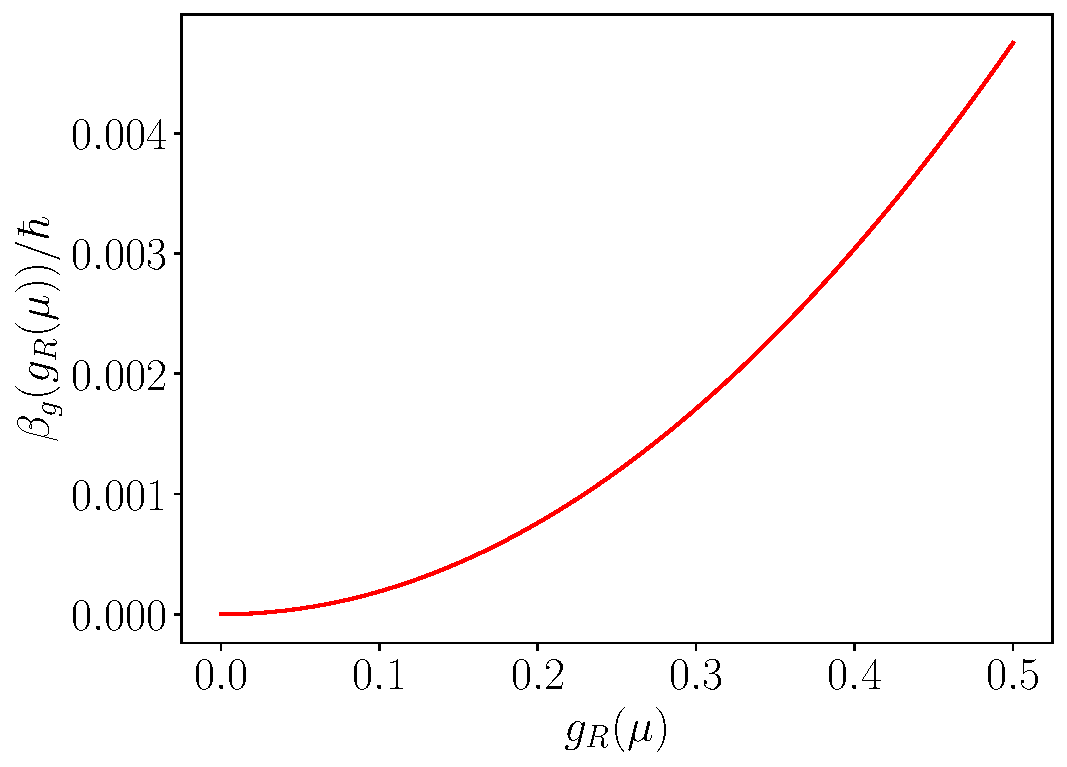
\includegraphics[scale=0.5]{C:/Users/pgraham1/Documents/GitHub/PSI/Quantum_Field_Theory_II/Homework2/TeX-JAM/beta.pdf}
    \caption{Beta function for the effective coupling $g_R$ at scale $\mu$ as a function of $g_R$ \label{fig1}}
  \end{figure}

  \item[(h)] In fig.\ref{fig1}, we see that the beta function for the effective coupling is positive and striclty increasing for $g_R > 0$. Since the beta function is a derivative of $g_R$ with respect to $\mu$, its positivity tells us that, as the energy momentum scale increases, the effective coupling also increases. At some point the increase in the effective coupling will break the assumption of small $g_R$ required for a good approximation of the beta function at $O(g_R^2)$ and further analysis will be required. If we decrease $\mu$, $g_R$ is reduced at a rate $\propto g_R^2$ (the decrease will slow down as $g_R = 0$ is approached). Going to low energy, we approach $g_R = 0$ (free theory). 
  
  \item[(i)] Using the decomposition of the action described above, we can perturbatively calculate the irreducible two-point function as 
  \begin{equation*}
    \begin{tikzpicture}[baseline=(current bounding box.center)]
      
      \begin{feynman}
        % External legs

        \vertex[label={left:$p$}]  (a) at (-1, 0);
        \vertex[label={right:$p$}] (b) at (1, 0);

        \vertex (v) at (0, 0);

        \fill (v) circle (2pt);

        %\fill (a) circle (2pt);
  
        \diagram* {
          (a) --[dashed]  (v),
          (b) --[dashed]  (v),
        };
      \end{feynman}
    \end{tikzpicture}
    + 
    \begin{tikzpicture}[baseline=(current bounding box.center)]
      
      \begin{feynman}
        % External legs

        \vertex[label={left:$p$}]  (a) at (-1, 0);
        \vertex[label={right:$p$}] (b) at (1, 0);

        \vertex (v) at (0, 0);

        \vertex (u) at (0, 1);

        \fill (v) circle (2pt);

        \draw[->] (-0.5, 0.7) arc (0:-180:-0.5cm) node [midway, label=above:$k$] {};

        %\fill (a) circle (2pt);
  
        \diagram* {
          (a) --[dashed] (v),
          (b) --[dashed] (v),
          (v) --[half right] (u),
          (u) --[half right] (v),
        };
      \end{feynman}
    \end{tikzpicture}
    +
    \begin{tikzpicture}[baseline=(current bounding box.center)]
     
      \begin{feynman}
        % External legs

        \vertex[label={left:$p$}]  (a) at (-1, 0);
        \vertex[label={right:$p$}] (b) at (1, 0);

        \vertex (v) at (0, 0);

        \draw (v) circle (3pt);

        %\fill (a) circle (2pt);
  
        \diagram* {
          (a) --[dashed] (v),
          (b) --[dashed] (v),
        };
      \end{feynman}
    \end{tikzpicture}
  \end{equation*}
  \begin{equation*}
    = \Gamma^{2}_R(p) = m_R^2 + p^2 + \hbar \frac{g_R}{2} T(m_R) + \hbar B_1 + O(\hbar^2)
  \end{equation*}
  where the full line represents a propagator associated to mass $m_R$ (in principle it involves the bare mass $m_R^2 + \hbar B_1$, but the counter term contribution is shifted out of the one-loop expansion by the factor of $\hbar$ from the loop) and the dashed lines are truncated propagators. A symmetry factor of $1/2$ is included for the loop diagram. The first and last terms are doubly truncated and are respectively associated to mass $m_R$ (marked with $\bullet$) and $\hbar B_1$ (marked with $\circ$). These two diagrams represent the bare mass doubly truncated propagator $m_R^2 + \hbar B_1 + p^2$. The loop integral $T$ is given by 
  \begin{align*}
    T(m_R) = \int \frac{\text{d}^4k}{(2\pi)^4} \frac{1}{k^2 + m_R^2} = \int \text{d}\Omega \int \frac{\text{d}k}{(2\pi)^4} \frac{k^3}{k^2 + m_R^2} = \frac{2}{(4\pi)^2} \int \text{d}k \frac{k^3}{k^2 + m_R^2}.  
  \end{align*}
  To UV regulate this integral, we introduce a sharp UV cutoff $\Lambda$ to get 
  \begin{align*}
    T(m_R, \Lambda) = \frac{2}{(4\pi)^2} \int_0^{\Lambda} \text{d}k \frac{k^3}{k^2 + m_R^2}.  
  \end{align*}
  \item[(j)] We take a detour to show how the $D$ dimensionnal angular integral $\int text{d}\Omega_D$ is evaluated. Consider the following Gaussian integral on $D$ real variables $x_i$:
  \begin{align*}
    I = \int_{-\infty}^{\infty} \text{d}x_1 \cdots \text{d}x_D \exp\left(-\sum_{i=1}^D x_i^{2}\right) = \prod_{i=1}^D\int_{-\infty}^{\infty} \text{d}x_i \exp\left(- x_i^{2}\right) = (\sqrt{\pi})^D.
  \end{align*}
  We can express this integral in a hyperspherical coordinate system with radius variable $r^2 = \sum_{i=1}^D x_i^2$ and angular variables associated to a measure $\text{d}\Omega_D$. It then reads 
  \begin{align*}
    I =\int \text{d}\Omega_D \int_{0}^{\infty} \text{d}r \ r^{D-1}  \exp\left(-r^2\right).
  \end{align*}
  To bring this result closer to the definition of the gamma function, we perform the change of variables $r^2 = u$ associated to $\text{d}r = \text{d}u/(2\sqrt{u})$ to obtain
  \begin{align*}
    I =\frac{1}{2}\int \text{d}\Omega_D \int_{0}^{\infty} \text{d}u \ u^{(D-1)/2-1/2}  \exp\left(-u\right) = \frac{1}{2} \int \text{d}\Omega_D \frac{1}{2}\int \text{d}\Omega_D \int_{0}^{\infty} \text{d}u \ u^{D/2 - 1}  \exp\left(-u\right) = \frac{1}{2} \int \text{d}\Omega_D \Gamma(D/2).
  \end{align*}
  Comparing this result with the direct gausian integral evaluation, we find
  \begin{align*}
    (\sqrt{\pi})^D = \frac{1}{2} \int \text{d}\Omega_D \Gamma(D/2) \iff \int \text{d}\Omega_D = \dfrac{2 \pi^{D/2}}{\Gamma(D/2)} =  2 \pi^2 \quad (D=4). 
  \end{align*}
  \newpage
  \item[(k)] We can now evaluate the $k$ remaining integral in $T(m_R, \Lambda)$ as follows
  \begin{align*}
    T(m_R, \Lambda) &= \frac{2}{(4\pi)^2} \int_0^{\Lambda} \text{d}k \frac{k^3}{k^2 + m_R^2}\\
    &= \frac{2}{(4\pi)^2} \int_{m_R^2}^{\Lambda^2 + m_R^2} \text{d}u \frac{u-m_R^2}{2u}, \quad \text{with} \quad u = k^2 + m_R^2, \quad \text{d}u/2 = k \ \text{d}k\\
    &= \frac{2}{(4\pi)^2} \left[\frac{1}{2}u - \frac{m_R^2}{2} \ln|u|\right]_{m_R^2}^{\Lambda^2 + m_R^2} = \frac{1}{(4\pi)^2} \left(\Lambda^2 - \frac{m_R^2}{2} \ln\left(\frac{\Lambda^2 + m_R^2}{m_R^2}\right)\right)\\& \sim \frac{1}{(4\pi)^2} \left(\Lambda^2 - m_R^2 \ln\left(\frac{\Lambda^2}{m_R^2}\right)\right)\quad (\Lambda/m_R \to \infty).
  \end{align*}
  We have identified two UV divergent terms: one is quadratic and the other is logarithmic.
  \item[(l)] We now impose that the two-point has a zero at $p^2 = -m_{p}^2$ where $m_{p}$ is the physical mass which is independant of the scale $\mu$ associated to $m_R$ and $g_R$. In the one-loop expression for the two-point function, $p$ only appears as a quadratic term. The positive zero of the two-point function is realised when $p^2$ equals the oposite of the remaining terms and these $p$-independant terms are therefore the physical mass squared. To extract them, we can set $p=0$ (we note that even if the coupling $g_R$ runs with change in scale, we are working at a fixed scale here and $g_R(\mu)$ is fixed). Setting $m_p = m_R$ at scale such that $\mu^2 = m_R^2 = (p_i^{\text{ref}})^2$ then corresponds to the condition
  \begin{align*}
    \Gamma^{2}_R(0, m_R(\mu), g_R(\mu), \mu) &= m_R^2 + \hbar \frac{g_R}{2} T(m_R) + \hbar B_1  = m_R^2\\
    & \iff B_1(m_R = \mu, g_R(\mu), \mu) = \frac{g_R(\mu)}{2} \frac{1}{(4\pi)^2} \left(-\Lambda^2 + \mu^2 \ln\left(\frac{\Lambda^2}{\mu^2}\right)\right).
  \end{align*}
  There are multiple choices of counter term that satisfy this condition. Imposing the decomposition $B_1 = B_{1, 0}(\mu, g_R, \Lambda) + m_R(\mu)^2 B_{1, 0}(\mu, g_R, \Lambda)$ linear in $m_R^2$ leads to the choice 
  \begin{align*}
    B_1 = \frac{g_R}{2} \frac{1}{(4\pi)^2} \left(-\Lambda^2 + m_R(\mu)^2 \ln\left(\frac{\Lambda^2}{\mu^2}\right)\right).
  \end{align*}
  \item[(m)] With the counter terms found in (l), the two-point function becomes
  \begin{align*}
    \Gamma^{2}_R(p, m_R(\mu), g_R(\mu), \mu) &= p^2 + m_R^2 + \hbar \frac{g_R}{2} \frac{1}{(4\pi)^2} \left(\Lambda^2 - m_R(\mu)^2 \ln\left(\frac{\Lambda^2}{m_R(\mu)^2}\right)\right) + \hbar \frac{g_R}{2} \frac{1}{(4\pi)^2} \left(-\Lambda^2 + m_R(\mu)^2 \ln\left(\frac{\Lambda^2}{\mu^2}\right)\right)\\
    &= p^2 + m_R^2 + \hbar \frac{g_R}{2} \frac{1}{(4\pi)^2} \left( m_R(\mu)^2 \ln\left(\frac{ m_R(\mu)^2}{\mu^2}\right)\right)
  \end{align*}
  which is UV finite since all dependance on the cutoff $\Lambda$ has been removed by the counterterm. We see that the limiting value of the two point function when $m_R \to 0$ is $0$ (we get the limit $\lim_{m_R \to 0} m_R^2 \ln (m_R^2/\mu^2) = 0$), and we conclude that the two-point function found is finite for all finite $m_R$ and $p$.
  \item[(n)] Since the two point-function values are independant of scale, given two scales $\mu'$ and $\mu$, we can write 
  \begin{align*}
    &\Gamma^{2}_R(p, m_R(\mu), g_R(\mu), \mu) = \Gamma^{2}_R(p, m_R(\mu'), g_R(\mu'), \mu')\\
    &\iff 
    p^2 + m_R(\mu)^2 + \hbar \frac{g_R(\mu)}{2} \frac{1}{(4\pi)^2} \left( m_R(\mu)^2 \ln\left(\frac{ m_R(\mu)^2}{\mu^2}\right)\right) = p^2 + m_R(\mu')^2 + \hbar \frac{g_R(\mu')}{2} \frac{1}{(4\pi)^2} \left( m_R(\mu')^2 \ln\left(\frac{ m_R(\mu')^2}{(\mu')^2}\right)\right)\\
    &\iff 0= m_R(\mu')^2 + \hbar \frac{1}{2(4\pi)^2} g_R(\mu') m_R(\mu')^2 \ln\left(\frac{ m_R(\mu')^2}{(\mu')^2}\right) - m_R(\mu)^2  - \hbar \frac{1}{2(4\pi)^2} g_R(\mu) m_R(\mu)^2 \ln\left(\frac{ m_R(\mu)^2}{\mu^2}\right)
  \end{align*}
  Supposing $m_R(\mu) = a(\mu', \mu) +  b(\mu', \mu)\hbar$ \footnote{Formaly this is a perturbative ansatz for a functional equation. It is justified by the fact $m_R(\mu)$ can be expressed as a function of $\mu'$ with a Taylor expansion $m_R(\mu) = m_R(\mu') + c(\mu')(\mu - \mu') + \cdots$ where the terms are also regrouped by powers of $\hbar$}, using $g_R(\mu) = g_R(\mu') + (\cdots)\hbar$ and keeping only terms up to $O(\hbar)$, we get 
  \begin{align*}
    &O(\hbar^0): \quad a(\mu', \mu)^2 = m_R(\mu')^2 \implies a(\mu') = \pm m_R(\mu') \quad \text{($+$ because $\hbar=0 \to$ classical solution $\to m_R(\mu) = m_R(\mu') = \text{cst}$)}\\
    &O(\hbar^1): \quad \hbar \frac{1}{2(4\pi)^2} g_R(\mu') m_R(\mu')^2 \ln\left(\frac{ m_R(\mu')^2}{(\mu')^2}\right) - 2\hbar m_R(\mu') b(\mu', \mu) - \hbar \frac{1}{2(4\pi)^2} g_R(\mu') m_R(\mu')^2 \ln\left(\frac{ m_R(\mu')^2}{\mu^2}\right)\\
    &\implies b(\mu', \mu) = \frac{1}{4(4\pi)^2} g_R(\mu') m_R(\mu') \ln\left(\frac{\mu^2}{(\mu')^2}\right),\ a(\mu', \mu) = m_R(\mu').  
  \end{align*}
  Combining the two orders studied, we have the relation $m_R(\mu) = m_R(\mu') + \hbar \frac{1}{4(4\pi)^2} g_R(\mu') m_R(\mu') \ln\left(\frac{\mu^2}{(\mu')^2}\right)$.
  \item[(o)] When $\mu = m_R$, the two-point function reduces to $\Gamma^{2}_R(p) = p^2 + m_R^2 + O(\hbar^2)$ and has a zero at $p^2 = -m_p^2 = -m_R^2$ implying that the renormalized mass coincides with the physical mass at this scale. 
  \item[(p)] Starting from the result found in (n) and setting the $\mu = \mu' +\delta \mu$ (with $\delta \mu$ small), the anomalous dimension $\gamma_{m^2}$ can be expressed as follows:
  \begin{align*}
    &m_R(\mu'+\delta \mu) - m_R(\mu') = \hbar \frac{1}{4(4\pi)^2} g_R(\mu') m_R(\mu') \ln\left(\frac{(\mu')^2 + 2 \mu' \delta \mu}{(\mu')^2}\right) = \hbar \frac{1}{4(4\pi)^2} g_R(\mu') m_R(\mu') \left(\frac{2\delta \mu}{\mu'}\right)\\
    &\implies \gamma_{m^2} := \mu' \frac{d \ln(m_R(\mu')^2)}{d \mu'}= \mu' \frac{2}{m_R(\mu')}\lim_{\delta\mu \to 0} \dfrac{m_R(\mu'+\delta \mu) - m_R(\mu')}{\delta \mu} = \hbar \frac{1}{(4\pi)^2} g_R(\mu')
  \end{align*}
\end{enumerate}


\section{Acknowledgement}

Thanks to Dan for guidance in the interview which is related to my answer to (f) and (n)




% References
\makereferences
%-------------------------------------------------------


%%%%%%%%%%%%%%%%%%%%%%%%
% Terminer le document %
%%%%%%%%%%%%%%%%%%%%%%%%
\end{document}
